\documentclass[12pt]{book}

\usepackage{amsmath, amsthm, mathtools, dsfont, amssymb, pifont}
\usepackage[mathscr]{euscript}
\usepackage[side,marginal, symbol, perpage]{footmisc}
\usepackage[left=1.5cm, right=6cm, top=2cm, bottom=2cm, marginparsep=0.75cm, marginparwidth=4cm]{geometry}

\usepackage{coursenotes}

\usepackage{multicol, booktabs, bm}

\setlength{\parskip}{1em}

\renewcommand{\theequation}{\thechapter.\arabic{equation}}

\renewcommand{\thefootnote}{\ding{110}}

\begin{document}

% \chapter{Limits}
%
% \section*{Introduction to The Derivative}

% \newpage

\section{Definitions of Limits}

\begin{defn}{Limit of a Function (Early Definition)}
  Suppose the function $f$ is defined for all $x$ near some value $a$ except possibly at $a$ itself.
  If $f(x)$ is arbitrarily close to some value $L$ whenever $x$ is sufficiently close to $a$ (without actually equaling it), then we write
  \[\lim_{x\to a} f(x) = L\]
\end{defn}

\begin{note}{Quick Notes} \hspace{1cm}
  \begin{itemize}
    \item Sometimes we'll write $f(x) \to L$ as $x\to a$.
    \item Limits do not have anything to do with function values, since it depends on values \textit{near} $a$.
    \item We can make $x$ ``get close to'' $a$ in two ways (from the left or from the right).
    \item We can investigate limits in three ways: graphically, numerically, and analytically.
  \end{itemize}
\end{note}

\begin{defn}{Graphically}
  As you ``move'' closer to the $x$-value on the graph that you care about, what is happening to the $y$-values?
  Notice that since we only ``get close'' to $a$, we don't care about the specific function value.
\end{defn}

\begin{defn}{Numerically}
  Pick $x$-values that are close to $a$ and create a table of values.
  What is the pattern?
\end{defn}

\section*{One-Sided Limits}

\begin{defn}{Right-Sided Limit}
  If $f$ is close to $L$ whenever $x$ is close to, but greater than, $a$, then we write:
  \[ \lim_{x\to a^+} f(x)=L\]
\end{defn}

\begin{defn}{Left-Sided Limit}
  If $f$ is close to $L$ whenever $x$ is close to, but less than, $a$, then we write:
  \[ \lim_{x\to a^-} f(x)=L\]
\end{defn}

\begin{thm}{Relationship Between One and Two-Sided Limits}
  Assume $f$ is defined for all $x$ near $a$ except possibly at $a$.
  Then $\dlim_{x\to a} f(x) = L$ if and only if $\dlim_{x\to a^-}f(x) = L = \dlim_{x\to a^+} f(x)$.
\end{thm}

\section*{Examples}

\begin{itemize}
  \item Graph a small piecewise function with a hole, but the limit existing.
  \item Graph a small piecewise function where the left side limit does not equal the right sided limit.
  \item Numerically find:
  \begin{multicols}{3}
    \begin{itemize}
      \item $\dlim_{x\to 4} \dfrac{x-4}{\sqrt{x}-2}$
      \item $\dlim_{x\to 1} \dfrac{\sqrt{x}-1}{x-1}$
      \item $\dlim_{x\to 2} \dfrac{x^3-8}{4(x-2)}$
    \end{itemize}
  \end{multicols}
  \item Examine $\dlim_{x\to 0} \cos\left(\dfrac{1}{x}\right)$.
  Numerically, it looks like $\dlim_{x\to 0} \cos\left(\dfrac{1}{x}\right)=-1$, but it actually oscillates between $-1$ and 1.

  Note that when $x=\dfrac{1}{n\pi}$, we can see that  $\cos\left(\dfrac{1}{x}\right)=\cos(n\pi)$.
  For bigger values of $n$, we know that $x=\dfrac{1}{n\pi} \to 0$, and we can also use some basic trig knowledge to analyze what happens when $n$ is odd and when $n$ is even.
  So as $n$ gets bigger, it bounces back and forth between even and odd values, meaning the value of $\cos(n\pi)$ oscillates between $-1$ and $1$.

  So, show that $\dlim_{x\to0^+}\cos(1/x)$ does not exist to show that the two-sided limit does not exist.
\end{itemize}

% \newpage
%
% \section{Properties of Limits}

\begin{recap}
  \begin{itemize}
    \item If $f(x)$ is arbitrarily close to $L$ whenever $x$ is sufficiently close to, \textit{but not equal to} $a$, then we say $\dlim_{x\to a}f(x) = L$.
    \item If the left-side limit and the right-side limit do not match up, we say that the (two-sided) limit does not exist.
    \item We can estimate limits numerically by evaluating $f$ at $x$-values close to (and on either side of) $a$.
    We look to see if the $y$-values are arbitrarily close to some real number.
    \item We can estimate limits graphically by visualizing the function values around $a$, and again trying to see if the $y$-values are arbitrarily close to some value.
  \end{itemize}
\end{recap}

We've estimated limits numerically and graphically, but these can be difficult without more tools at our disposal.
Here we'll build up some analytic methods of evaluating limits.
We'll start by analyzing two specific functions, and build two limit laws for those specific functions.

Then, we'll build some general limit laws for any function.

To start, then, two easy limits.

\subsection*{Two Easy Limits}
\begin{enumerate}
  \item Let $f(x) = k$, where $k$ is some real number.
  Then $\dlim_{x\to a} k = k$.

  \begin{describe}{\textit{Explanation}}
    This function is a constant function, meaning that every output of the function is $k$, no matter what the input is.\\

    That means that for every $x$, $f(x) = k$. So then for all $x$ that are close to $a$, $f(x) = k$.\\

    So $f(x)$ is arbitrarily close to $k$ (in fact, it's equal to $k$) for all $x$ sufficiently close to, but not equal to, $a$.\\

    Visually, we can see some graphical evidence of this.
    \begin{figure}[h!tb]
      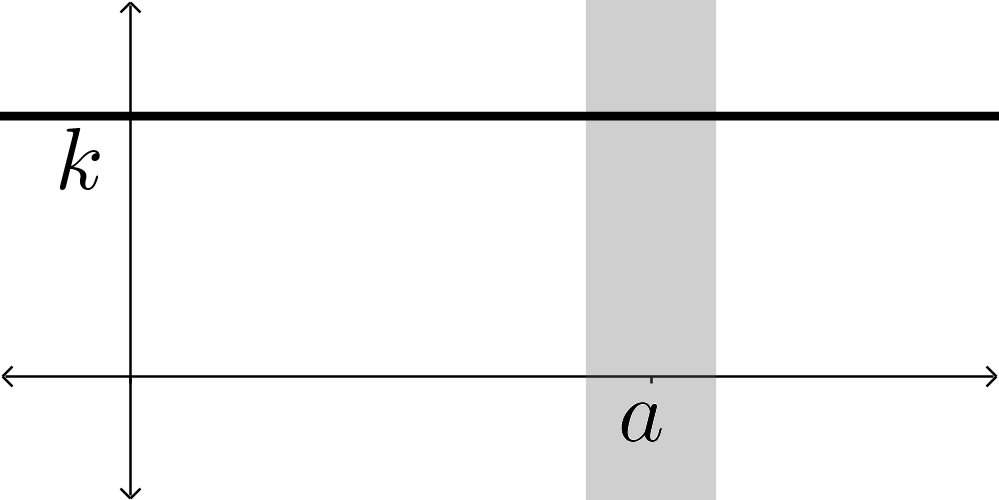
\includegraphics[scale=0.5]{./1_limits/images/1-2_graph1.png}
      \centering
    \end{figure}
  \end{describe}
  \item Let $f(x) = x$. Then $\dlim_{x\to a} x = a$.

  \begin{describe}{\textit{Explanation}}
    This function is the identity function, meaning that every output of the function is the same as the input.\\

    Then, when $x$ is close to $a$, $f(x) = x$ is also close to $a$.
    In fact, $f(x)$ is as close to $a$ as $x$ is, since they're the same thing.
    Thus, $f(x)$ is arbitrarily close to $a$ whenever $x$ is sufficiently close to $a$.\\

    Visually, we can see some graphical evidence of this.
    \begin{figure}[h!tb]
      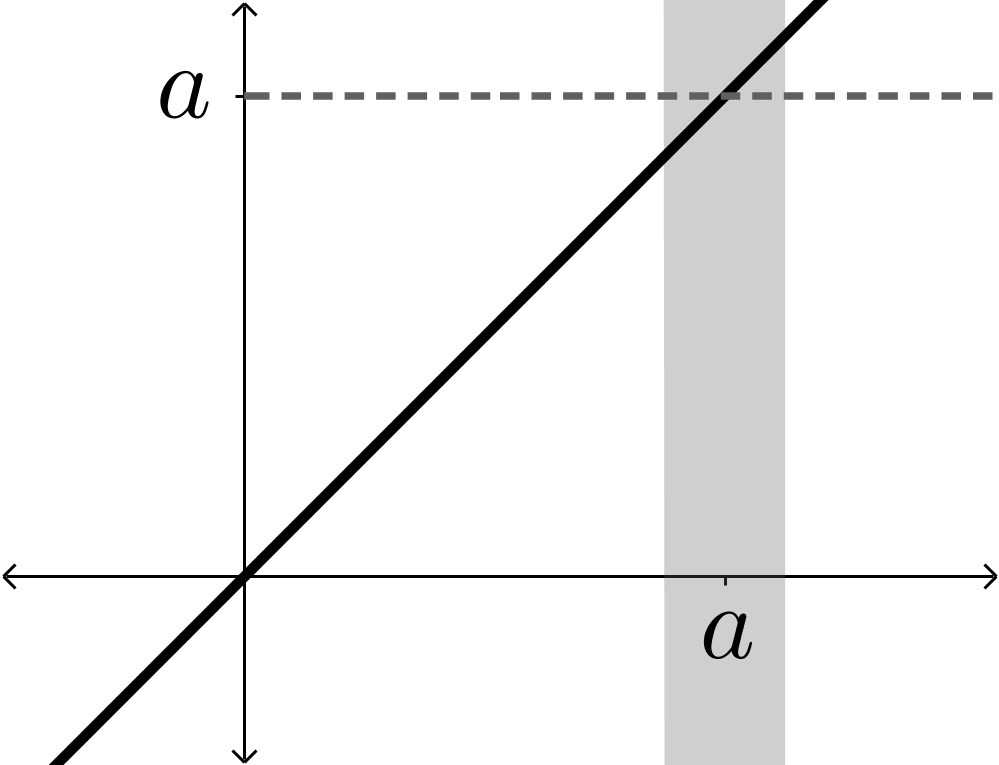
\includegraphics[scale=0.5]{./1_limits/images/1-2_graph2.png}
      \centering
    \end{figure}
  \end{describe}
\end{enumerate}

\begin{note}{Examples}
  There really isn't much to do here, since once you've seen a couple of these examples, you've essentially seen them all.

  \begin{enumerate}
    \item $\dlim_{x\to 4} -3 = -3$
    \item $\dlim_{x\to -8} 7 = 7$
    \item $\dlim_{x\to -1} x = -1$
    \item $\dlim_{x\to 15} x = 15$
  \end{enumerate}
\end{note}

\subsection*{Limit Laws In General}

We will now think about functions in general, and build some laws/properties to apply to limits, no matter the context.
These properties will all be based around some basic operations on functions: addition, multiplication, division, and some exponents.

\begin{imp}{Limit Laws and Properties}
  Let $f$ and $g$ be two functions, and assume that $\dlim_{x\to a} f(x)$ and $\dlim_{x\to a} g(x)$ both exist.
  Then:
  \begin{enumerate}
    \item $\dlim_{x\to a} [f(x)\pm g(x)] = \lim_{x\to a} f(x) \pm \lim_{x\to a} g(x)$
    \item $\dlim_{x\to a} cf(x) = c\lim_{x\to a} f(x)$ for any constant multiple (coefficient) $c$.
    \item $\dlim_{x\to a} [f(x)\cdot g(x)] = \left[\lim_{x\to a} f(x)\right] \left[\lim_{x\to a} g(x)\right]$
    \item $\dlim_{x\to a} \frac{f(x)}{g(x)} = \frac{\dlim_{x\to a} f(x)}{\dlim_{x\to a} g(x)}$ if $\dlim_{x\to a} g(x)\neq0$
    \item $\dlim_{x\to a} (f(x))^n = \left(\dlim_{x\to a} f(x) \right)^n$ for positive integers $n$.
  \end{enumerate}
\end{imp}

\begin{note}{Explanations}\hspace{1cm}
  \begin{enumerate}
    \item We should be able to rationalize this property, since $(f\pm g)(x)= f(x)\pm g(x)$.
    Since the limit is concerned with what the $y$-value is arbitrarily close to, we can see that the operation is ``preserved" across the limit.
    The following saying is helpful here: ``the limit of a sum (or difference) is the sum (or difference) of the limits.''
    \item Notice that a coefficient really represents repeated addition: $c\cdot f(x) = \underbrace{f(x) + f(x) + ...+ f(x)}_{c \text{ times}}$.
    \item ``The limit of a product is the product of the limits.''
    Limits preserve multiplication in the same way that they preserve sums.
    \item Dividing is really just multiplication by a reciprocal.
    The only thing we need to worry about is dividing by 0.\footnote{We'll investigate this more!}
    \item An exponent really represents repeated multiplication: $(f(x))^n = \underbrace{f(x) \cdot f(x) \cdot ... \cdot f(x)}_{n \text{ times}}$.
  \end{enumerate}
\end{note}

\subsection*{Examples}
Given $\dlim_{x\to 1} f(x) = 4$ and $\dlim_{x\to 1} g(x) = 2$, evaluate the following limits:
\begin{enumerate}
  \item $\dlim_{x\to 1}\left(\dfrac{f(x)-g(x)}{f(x)}\right)$

  When we consider $\dlim_{x\to 1}\left(\dfrac{f(x)-g(x)}{f(x)}\right)$, we should notice that the function $\dfrac{f(x)-g(x)}{f(x)}$ is really a combination of the two functions that we have information about.
  The operations are subtraction and division.
  We can use the properties above to re-write this limit:

  \begin{align*}
    \lim_{x\to 1}\left(\dfrac{f(x)-g(x)}{f(x)}\right) &= \frac{\dlim_{x\to 1} (f(x)-g(x))}{\dlim_{x\to 1} f(x)} & \text{Division Property (Property 4)}\\
    & = \frac{\left(\dlim_{x\to 1} f(x)\right)- \left(\dlim_{x\to 1} g(x)\right)}{\dlim_{x\to 1} f(x)} & \text{Difference Property (Property 1)}
  \end{align*}

  Now, we notice that we can input the values above, since we know that $\dlim_{x\to1} f(x) = 4$\footnote{Notice that since $\dlim_{x\to1}f(x)\neq0$, we're allowed to put this value in the denominator. Remember, we can't evaluate a limit using these properties if there's division by 0.} and $\dlim_{x\to 1}g(x) = 2$.

  \begin{align*}
    \frac{\left(\dlim_{x\to 1} f(x)\right)- \left(\dlim_{x\to 1} g(x)\right)}{\dlim_{x\to 1} f(x)} & = \frac{4-2}{4}\\
    &= \frac{2}{4} = \frac12
  \end{align*}

  So we can see that $\dlim_{x\to 1}\left(\dfrac{f(x)-g(x)}{f(x)}\right) = \frac{1}{2}$.

  \item $\dlim_{x\to 1} \left(3f(x)+\dfrac{2(g(x))^3}{5}\right)$

  Here, we have two functions added together, an exponent on one, and coefficients on each. We can again use the properties above.
  Again, we'll use the properties above:

  \begin{align*}
    \dlim_{x\to 1} \bigg( 3f(x) &\left.+\dfrac{2(g(x))^3}{5}\right) \\
    & = \left(\dlim_{x\to 1} 3f(x)\right) + \left(\dfrac{2(g(x))^3}{5}\right) & \text{Sum Property (Property 1)}\\
    &= 3\left(\dlim_{x\to 1} f(x)\right) + \dfrac{2}{5}\left(\dlim_{x\to1} (g(x))^3 \right) & \text{Coefficient Property (Property 2)}\\
    & = 3\left(\dlim_{x\to 1} f(x)\right) + \dfrac{2}{5}\left(\dlim_{x\to 1}g(x)\right)^3 & \text{Exponent Property (Property 5)}
  \end{align*}

  Again, we can input the values above, since $\dlim_{x\to1} f(x) = 4$ and $\dlim_{x\to 1}g(x) = 2$ are given.

  \begin{align*}
    3\left(\dlim_{x\to 1} f(x)\right) + \dfrac{2}{5}\left(\dlim_{x\to 1}g(x)\right)^3 & =3(4) + \dfrac{2}{5}(2)^3 \\
    &= 12 + \dfrac{2}{5}(8) = 12 + \dfrac{16}{5}\\
    & = \dfrac{76}{5}
  \end{align*}

  So the limit $\dlim_{x\to 1} \left(3f(x)+\dfrac{2(g(x))^3}{5}\right) = \dfrac{76}{5}$.
\end{enumerate}

We can see that these limit laws are very helpful for building our limit ``piece-by-piece.''
What happens, though, when we have some function or combination of functions that involves an operation or function type that is not covered in these properties?
What about functions involving trigonometric functions, exponentials, logarithms, etc.?
What about exponents that are not integers?
We'll investigate square roots next.
\begin{note}{Remember}
  Roots and radicals can be written as fraction exponents.
  \[\sqrt{x} = x^{1/2}\]
\end{note}

\subsection*{Square Roots}

Let's consider the function $y=\sqrt{x}$.
Specifically, we'll consider $\dlim_{x\to 0} \sqrt{x}$.

In the spirit of this chapter, we should start with numerical and graphical esimations.

\subsubsection*{Graphical Approximation}

Let's consider the graph of $y=\sqrt{x}$ around $x=0$.

% Image of graph.



\subsubsection*{Numerical Approximation}

\textbf{Left-Sided Limit}

\begin{tabular}{ccccc} \toprule
  $\bm{x}$ & $-0.5$ & $-0.1$ & $-0.01$ & $-0.001$ \\ \midrule
  $\bm{\sqrt{x}}$ & $\sqrt{-0.5}$ & $\sqrt{-0.1}$ & $\sqrt{-0.01}$ & $\sqrt{-0.001}$\\ \bottomrule
\end{tabular}

\begin{flushright}
  \textbf{Right-Sided Limit}

  \begin{tabular}{ccccc} \toprule
    $0.001$ & $0.01$ & $0.1$ & $0.5$ & $\bm{x}$ \\ \midrule
    $\sqrt{0.001}$ & $\sqrt{0.01}$ & $\sqrt{0.1}$ & $\sqrt{0.5}$ & $\bm{\sqrt{x}}$ \\ \bottomrule
  \end{tabular}
\end{flushright}

We should notice the strange behavior here, specifically with the left-sided limit.

None of those outputs are real numbers.
Strange.

On a different note, the right-sided limit looks like it's approaching 0.
All of those square roots are getting progressively smaller as $x$ gets closer to 0.

% \newpage
%
% \section{Techniques for Evaluating Limits}


\begin{note}{Examples}
Notice that polynomials and rational functions become kind of easy:
\begin{enumerate}
\item $\dlim_{x\to 4}x^3-5x^2+3x-4$
\item $\dlim_{x\to -2} \dfrac{x^2+1}{x^2-5x-1}$
\end{enumerate}
\end{note}

Essentially, we're able to just plug values in for any polynomial function or rational function. When might this screw up for rational functions?

\newpage
\begin{thm}{Limits of Polynomial and Rational Functions}
Let $p$ and $q$ be polynomials and let $a$ be some constant.
Then:

\begin{itemize}
\item $\dlim_{x\to a} p(x) = p(a)$
\item $\dlim_{x\to a} \dfrac{p(x)}{q(x)} = \dfrac{p(a)}{q(a)}$ as long as $q(a)\neq 0$
\end{itemize}
\end{thm}

So, what happens when $\dlim_{x\to a} f(x) \neq f(a)$? What if we have a rational function that does not exist at a certain point?

\begin{note}{Remember}
The limit of $f(x)$ as $x\to a$ does not depend on the actual function value at $x=a$.
\end{note}

\begin{note}{Examples}
\begin{multicols}{2}
\begin{enumerate}
\item $\dlim_{x\to2} \dfrac{x^2-6x+8}{x^2-4}$
\item $\dlim_{x\to1} \dfrac{\sqrt{x}-1}{x-1}$
\end{enumerate}
\end{multicols}
\end{note}

\subsection*{Reality Check}

We've got some tools to evaluate limits analytically, and that's great. We probably feel pretty good. Limits aren't so bad! But there are still some important limits that we'll struggle with analytically.

\begin{note}{Example}
Estimate the slope of the line tangent to $f(x) = 2^x$ at point $(0,1)$.\\

Just like we did to start the semester, we'll need to set up the slope of a secant line between some point $(x, 2^x)$ and our point $(0,1)$. Then we can take a limit as $x\to0$: $\dlim_{x\to0} \dfrac{2^x-1}{x}$.\\

Technically we need to check both sides of the limit, but let's just check one side numerically. Set up a chart with values for $x$.
\end{note}

\section*{The Squeeze Theorem}

This will be another tool for calculating tricky limits. Essentially what we'll do is try to trap (or squeeze) our function in between two other functions that have the same limit as $x\to a$. Then we'll know the limit of our function as $x \to a$.

\begin{thm}{The Squeeze Theorem}
Assume fucntions $f$, $g$, and $h$ satisfy $f(x) \leq g(x) \leq h(x)$ for all values of $x$ near $a$ (except possibly at $a$ itself). If $\dlim_{x\to a} f(x) = \dlim_{x\to a} h(x) = L$, then $\dlim_{x\to a} g(x) = L$ also.
\end{thm}

\begin{itemize}
\item Squeeze $g(x) = \sin x$ between $f(x) =-|x|$ and $g(x) = |x|$ for $x\to 0$.
\item Squeeze $g(x) = \cos x$ between $f(x) =1$ and $g(x) = |x|+1$ for $x\to 0$.
\begin{note}{Note}
Shift everything down 1 unit if it's easier.
\end{note}
\end{itemize}

\newpage
\begin{note}{Example}
Use the Squeeze Theorem to find the limit $\dlim_{x\to 0} x^2\sin(1/x)$.\\

The first problem is to think about which functions to use. This isn't always easy. We need a function that is greater than $x^2\sin(1/x)$ around $x=0$ and a function that is less than $x^2\sin(1/x)$ around $x=0$.

\textbf{\textit{Notice:}} We can put some inequalities around trig functions that might help. For any angle $\theta$, we know that $-1\leq \sin \theta \leq 1$. So if the angle $\theta = 1/x$, then we know that $-1\leq \sin(1/x) \leq 1$.\\

So $-x^2 \leq x^2 \sin (1/x) \leq x^2$. This makes things REALLY easy!
\[-x^2 \leq x^2 \sin (1/x) \leq x^2 \to \dlim_{x\to0} -x^2 \leq \dlim_{x\to0} x^2 \sin (1/x) \leq \dlim_{x\to0} x^2\]

But we know that $\dlim_{x\to0} -x^2 = \dlim_{x\to0} x^2 = 0$. So $0\leq \dlim_{x\to0} x^2 \sin (1/x) \leq 0$ which tells us that $\dlim_{x\to0} x^2 \sin (1/x)=0$.
\end{note}

% \newpage
%
% \section{Infinite Limits}


Two types of limits: infinite limits and limits at infinity.

\subsection*{Infinite Limits}

\textit{Look at the graph of $f(x) = \dfrac{1}{x-1}$. Find $\dlim_{x\to1^+} f(x)$.}

Since the graph diverges off to infinity as $x\to1^+$, we say that $\dlim_{x\to1^+} \frac{1}{x-1} = \infty$ or that $f(x) = \dfrac{1}{x-1}\to \infty$ as $x\to 1^+$.
\textbf{Be careful} with this notation - make note that since $\infty \notin \mathbb{R}$, the limit doesn't actually exist even though we're saying it is equal to infinity.
Really what we're doing is using the symbol $\infty$ to describe the way in which the limit fails to exist.

\begin{note}{Note}
  If we change the limit to approach 1 from the left, we get the result $\dlim_{x\to1^-} \frac{1}{x-1} = -\infty$.

  Does $\dlim_{x\to 1} \frac{1}{x-1}$ exist?
  Can we describe it using $\infty$?
  What if we were looking for $\dlim_{x\to1} \frac{1}{(x-1)^2}$?
  Since both the left and right sided limits $\to \infty$, we can say that $\dlim_{x\to1} \frac{1}{(x-1)^2}=\infty$.
  Again, this limit does not exist, but we can still use notation to explain its behavior.
\end{note}

\begin{defn}{One-Sided Infinite Limits}
  Suppose $f$ is defined for all $x$ near $a$ where $x>a$.
  If $f(x)$ because arbitrarily large for all $x$ sufficiently close to (but greater than) $a$, we say $\dlim_{x\to a^+}f(x)=\infty$.

  The rest of the one-sided limits, $\dlim_{x\to a^+}f(x)=-\infty$, $\dlim_{x\to a^-}f(x)=\infty$, and $\dlim_{x\to a^-}f(x)=-\infty$ all act similarly.
\end{defn}

Each of these infinite limts represent \textbf{vertical asymptotes}.

\subsection*{Finding Infinite Limits Analytically}

The main thing that we can notice here is that when we have rational functions in the form $f(x)=a/b$, the function value will grow arbitrarily large in size (positive or negative) if $a$ stays relatively constant and $b$ approaches 0.

Finding out if the limit diverges to $\infty$ or $-\infty$ is as easy as checking signs on one sided limits.

\begin{note}{Examples}
  Find the vertical asymptote and analyze both one-sided limits at the asymptote for the following functions:
  \begin{multicols}{2}
    \begin{enumerate}
      \item $f(x) = \dfrac{2-5x}{x-3}$
      \item $f(x) = \dfrac{x^2-4x+3}{x^2-1}$
    \end{enumerate}
  \end{multicols}
\end{note}

\begin{note}{Another Example}
  Analyze the following one-sided limits:
  \begin{multicols}{2}
    \begin{enumerate}
      \item $\dlim_{\theta\to0^+} \cot \theta$
      \item $\dlim_{\theta\to0^-} \cot \theta$
    \end{enumerate}
  \end{multicols}
  Remember that $\cot \theta = \cos \theta / \sin \theta$.
\end{note}

% \newpage
%
% \section{Limits at Infinity}

We can also use $\infty$ as a symbol to indicate that the independent variable is either increasing or decreasing without bound: $x\to\infty$ and $x\to-\infty$.
Essentially, this limit gets at the end behavior of a function.

\begin{defn}{Limits at Infinity}
  If $f(x)$ becomes arbitrarily close to a finite number $L$ for all sufficiently large and positive (or negative) $x$, then we write
  \[ \lim_{x\to\pm\infty}f(x)=L.\]
  In either case, the line $y=L$ is a \textbf{horizontal asymptote}.
\end{defn}

\begin{note}{Example}
  We know that $f(x)=\arctan(x)$ (or $f(x)=\tan^{-1}(x)$) has horizontal asymptotes at $y=\pm \pi/2$.
  What limit statements represent those asymptotes?
  \[\lim_{x\to-\infty}\tan^{-1}(x)=-\pi/2 \hspace{2cm} \lim_{x\to\infty}\tan^{-1}(x)=\pi/2\]
\end{note}

\begin{note}{Try Some More}
  Evaluate the following limits:
  \begin{multicols}{3}
    \begin{enumerate}
      \item $\dlim_{x\to-\infty} \left( 2+\dfrac{10}{x^2}\right)$
      \item $\dlim_{x\to\infty} \left(5+\dfrac{\sin x}{\sqrt{x}}\right)$
      \item $\dlim_{x\to\infty} \left(\dfrac{x+6}{x^2-5x}\right)$
    \end{enumerate}
  \end{multicols}
\end{note}

What happens if there isn't a horizontal asymptote?

\begin{defn}{Infinite Limits at Infinity}
  If $f(x)$ becomes arbitrarily small/large as $x$ becomes arbitrarily small/large, then we write $\dlim_{x\to\pm\infty}f(x)=\pm\infty$.
\end{defn}

There may be other ways that these limits at infinity do not exist.
Consider: $\dlim_{x\to\infty} \sin x$.

\begin{thm}{Limits at Infinity of Powers and Polynomials}
Let $n$ be a positive integer and let $p$ be the polynomial $p(x)=a_nx^n+a_{n-1}x^{n-1}+\cdots+a_2x^2+a_1x+a_0$ where $a_n\neq0$.
\begin{enumerate}
  \item $\dlim_{x\to\pm\infty}x^n=\infty$ when $n$ is even
  \item $\dlim_{x\to\infty}x^n=\infty$ and $\dlim_{x\to-\infty}x^n=-\infty$ when $n$ is odd
  \item $\dlim_{x\to\pm\infty}x^{-n}=\dlim_{x\to\pm\infty}\dfrac{1}{x^n}$
    \item $\dlim_{x\to\pm\infty} p(x)=\dlim_{x\to\pm\infty} a_nx^n = \pm\infty$ depending on degree and leading coefficient.
  \end{enumerate}
\end{thm}

\begin{prf}{Part 4}
  Consider the polynomial $p(x) =a_nx^n+a_{n-1}x^{n-1}+\cdots+a_2x^2+a_1x+a_0$ where $a_n\neq0$.
  Factor $x^n$ out:
  \begin{align*}
    p(x) &= x^n\left(a_n+a_{n-1}\dfrac{x^{n-1}}{x^n}+ \cdots + a_2\dfrac{x^2}{x^n} + a_1\dfrac{x}{x^n}+a_0\dfrac{1}{x^n}\right)\\
    &= x^n\left(a_n+\dfrac{a_{n-1}}{x}+ \cdots + \dfrac{a_2}{x^{n-2}} + \dfrac{a_1}{x^{n-1}}+\dfrac{a_0}{x^n}\right)
  \end{align*}

  Take a limit of $p(x)$ as $x\to\pm\infty$:

  \begin{align*}
    \dlim_{x\to\pm\infty}p(x) & = \dlim_{x\to\pm\infty} x^n\left(a_n+\dfrac{a_{n-1}}{x}+ \cdots + \dfrac{a_2}{x^{n-2}} + \dfrac{a_1}{x^{n-1}}+\dfrac{a_0}{x^n}\right)\\
    &= \dlim_{x\to\pm\infty} x^n \cdot \dlim_{x\to\pm\infty} \left(a_n+\dfrac{a_{n-1}}{x}+ \cdots + \dfrac{a_2}{x^{n-2}} + \dfrac{a_1}{x^{n-1}}+\dfrac{a_0}{x^n}\right)\\
    & =  \dlim_{x\to\pm\infty} x^n \cdot \dlim_{x\to\pm\infty} (a_n)\\
    & = \dlim_{x\to\pm\infty} a_n x^n
  \end{align*}
  Note that each rational function $\to 0$ due to the third statement in the above theorem.
  Thus, only the first term has any impact on the limit of a polynomial.
\end{prf}

This is is a proof of something we've known for a while: we can judge the end behavior of a polynomial by the degree and the sign of the leading coefficient.
\begin{center}
  \begin{tabular}{ccc}
      & \textbf{Even} &   \textbf{Odd}\\
    \textbf{Positive} & $\nwarrow \nearrow$ & $\swarrow \nearrow$\\
    \textbf{Negative} & $\swarrow \searrow$ & $\nwarrow \searrow$
  \end{tabular}
\end{center}

\begin{thm}{End Behavior for Rational Functions}
  Suppose $f(x)=\dfrac{p(x)}{q(x)}$ is a rational function where:

  $p(x) = a_mx^m+a_{m-1}x^{m-1}+\cdots+a_2x^2+a_1x+a_0$ and

  $q(x) = b_nx^n+b_{n-1}x^{n-1}+\cdots+b_2x^2+b_1x+b_0$

  Then we have a few cases/possibilities:
  \begin{enumerate}
    \item If $m<n$, then $\dlim_{x\to\pm\infty} f(x)=0$, which means that $y=0$ is a horizontal asymptote.
    \item If $m=n$, then $\dlim_{x\to\pm\infty} f(x) = \dfrac{a_m}{b_n}$ (and so there is a horizontal asymptote again).
    \item If $m>n$, then $\dlim_{x\to\pm\infty} f(x)=\pm\infty$, which means that is no horizontal asymptote. We can figure out the limit by investigating $\dlim_{x\to\pm\infty} \dfrac{a_m}{b_n} x^{m-n}$.
    \begin{itemize}
      \item If $m=n+1$, then there is an oblique or slant asymptote.
    \end{itemize}
  \end{enumerate}
\end{thm}

Most of this is stuff we already knew from algebra.
Now, though, we don't need to worry about the specific cases.
We can just apply the theorem about polynomials to the numerator and denominator to investigate the new limit.

One of the weird things we did in Algebra was finding oblique or slant asymptotes.

\subsection*{Slant Asymptotes}

We noticed that slant or oblique asymptotes show up when the degree on top of the rational function was larger than the degree on the bottom by one.

EX: $f(x)=\dfrac{2x^2+6x-2}{x+1}$.

We used long division and then disregarded the remainder.
Here's why:

$f(x) = \dfrac{2x^2+6x-2}{x+1} = 2x+4- \dfrac{6}{x+1}$

$\dlim_{x\to\infty} f(x) = \dlim_{x\to\infty} 2x+4- \dfrac{6}{x+1} = (2x+4)-(0)$

So the ``end behavior'' of this rational function is really just the linear piece, since the limit of the remainder will just go to 0 anyways.
What happens in the degree on top is bigger by 2? More?

\subsection*{Some More Weird Limits at Infinity}

Rational functions like the ones we've seen are relatively familiar, but what happens when we move away from rational functions into similar types of functions?

\begin{note}{Example}
  Determine the end behavior of
  \[f(x) = \frac{8x^3-4x^2+5x-1}{\sqrt{4x^6+2x^4+1}}.\]

  Let's treat each ``end'' separately.
  We'll look at $\dlim_{x\to\infty}f(x)$ first before we look at $\dlim_{x\to-\infty}f(x)$.

  $\dlim_{x\to\infty} \frac{8x^3-4x^2+5x-1}{\sqrt{4x^6+2x^4+1}}$

  We have to be careful about the denominator, since the square root can mess things up.
  Since $x\to\infty$, we know that $x>0$, so we don't need to worry about square roots of negatives.
  \begin{align*}
    \dlim_{x\to\infty} \frac{8x^3-4x^2+5x-1}{\sqrt{4x^6+2x^4+1}}&= \frac{\dlim_{x\to\infty}8x^3-4x^2+5x-1}{\dlim_{x\to\infty}\sqrt{4x^6+2x^4+1}}\\
    & = \frac{\dlim_{x\to\infty}8x^3}{\sqrt{\dlim_{x\to\infty}4x^6+2x^4+1}}\\
    & =\dfrac{\dlim_{x\to\infty}8x^3}{\sqrt{\dlim_{x\to\infty}4x^6}}\\
    & = \dfrac{\dlim_{x\to\infty}8x^3}{\dlim_{x\to\infty}\sqrt{4x^6}}\\
    & = \frac{\dlim_{x\to\infty}8x^3}{\sqrt{\dlim_{x\to\infty}4x^6+2x^4+1}}\\
    & =\dfrac{\dlim_{x\to\infty}8x^3}{\sqrt{\dlim_{x\to\infty}4x^6}}\\
    & = \dfrac{\dlim_{x\to\infty}8x^3}{\dlim_{x\to\infty}\sqrt{4x^6}}\\
    & = \dfrac{\dlim_{x\to\infty}8x^3}{\dlim_{x\to\infty}2x^3}\\
    & = \dlim_{x\to\infty} \dfrac{8x^3}{2x^3} = \dlim_{x\to\infty} 4 = 4
  \end{align*}

  So we've found, through a lot of manipulation of limits, that $\dlim_{x\to\infty} f(x) = 4$.

  Let's check out the other side: $\dlim_{x\to-\infty} \frac{8x^3-4x^2+5x-1}{\sqrt{4x^6+2x^4+1}}$.

  Again, we need to be careful about the denominator.
  Since $x\to-\infty$, we know that $x<0$.
  Since all of the exponents under the square root are even, notice that the radicand will be positive (since negative numbers multiplied an even number of times will be positive).
  That's a good thing! No problems!
  We'll keep in mind, though, that the denominator will be positive.

  \begin{align*}
    \dlim_{x\to-\infty} \frac{8x^3-4x^2+5x-1}{\sqrt{4x^6+2x^4+1}} &= \dfrac{\dlim_{x\to-\infty}8x^3-4z^2+5x-1}{\dlim_{x\to-\infty}\sqrt{4x^6+2x^4+1}}\\
    & = \dfrac{\dlim_{x\to-\infty} 8x^3}{\sqrt{\dlim_{x\to-\infty} 4x^6-2x^4+1}}\\
    & = \dfrac{\dlim_{x\to-\infty} 8x^3}{\sqrt{\dlim_{x\to-\infty}4x^6}}
  \end{align*}

  \textbf{NOTE:} Before we move forward and get sloppy, notice that the square root (denominator) will be positive.
  When we pull the square root apart, if we leave $x\to-\infty$ when we bring it out, it'll become negative.
  So let's change the denominator: $\sqrt{\dlim_{x\to-\infty}4x^6} = \dlim_{x\to\infty}2x^3$.

  If we want to do the same trick as before where we bring the limit to the front of the fraction, they need to be the same limit.
  So we need to change the numerator too. $\dlim_{x\to-\infty} 8x^3 = \dlim_{x\to\infty}-8x^3$.

  So our limit with these changes: $\dfrac{\dlim_{x\to\infty}-8x^3}{\dlim_{x\to\infty}2x^3}$.
  We can go from here now easily.

  \[\dlim_{x\to\infty}\dfrac{-8x^3}{2x^3}=\dlim_{x\to\infty}-4=-4\]

  So we've found, through some weird manipulation of limits, that $\dlim_{x\to-\infty} f(x) = -4$.
\end{note}

Our textbook uses a different method in an example similar to this (Example 5).
Division and factoring.
If they want to see it again, try it with any other weird functions with square roots.

\begin{defn}{End Behavior of Some Transcendental Functions} \hspace{2cm}
  \begin{multicols}{2}
    $\dlim_{x\to \infty} e^x = \infty$

    $\dlim_{x\to \infty} e^{-x} = 0$

    $\dlim_{x\to \infty} \ln x = \infty$

    $\dlim_{x\to -\infty} e^x = 0$

    $\dlim_{x\to -\infty} e^{-x} = \infty$

    $\dlim_{x\to 0^+} \ln x = -\infty$
  \end{multicols}
\end{defn}

Note that some trig functions have some strange nonexistent limits at infinity.

\textbf{Example:} $\dlim_{x\to\pm\infty} \sin x$ does not exist

\subsection*{Squeeze Theorem Example}

Find $\dlim_{x\to\infty}\dfrac{\cos^2(2x)}{3-2x}$.
 Note that $0\leq \cos^2(2x)\leq 1$ for all $x$.

 \begin{align*}
   \dfrac{0}{3-2x} &\leq \dfrac{\cos^2(2x)}{3-2x}\leq\dfrac{1}{3-2x}
   0 &\leq \dfrac{\cos^2(2x)}{3-2x} \leq \dfrac{1}{3-2x}
   \dlim_{x\to\infty} 0 &= 0 = \dlim_{x\to\infty} \dfrac{1}{3-2x}
 \end{align*}

So by the Squeeze Theorem, $\dlim_{x\to\infty} \dfrac{\cos^2(2x)}{3-2x}=0$

% \newpage
%
% \section{Continuity}

Earlier, we classified polynomial and rational functions as ``easy'' limits (we could just check the function outputs for the limits). We'll expand that definition of ``easy'' limits here with a more formal definition of continuity.\\

What does continuity mean? What does it look like? What does it look like to ``break'' continuity?

\begin{defn}{Continuity at a Point}
A function is continuous at a point $a$ if $\dlim_{x\to a}f(x) = f(a)$. If this equality doesn't hold, we'll call $a$ a \textbf{point of discontinuity}.
\end{defn}

\begin{note}{Note}
The the continuity limit equality to hold, we need three things to be true:
\begin{enumerate}
  \item $f(a)$ is defined ($a$ is in the domain of $f$)
  \item $\dlim_{x\to a}f(x)$ exists ($\dlim_{x\to a^-} f(x) = \dlim_{x\to a^+} f(x)$)
  \item $\dlim_{x\to a}f(x) = f(a)$ (limit and function value are the same).
\end{enumerate}
\end{note}

This definition is a lot more robust than it seems. Using limits to define continuity adds a lot of depth to a concept that we don't normally consider that interesting.\\

\textit{Have students design functions that are either weird looking but continuous or break the definition of continuity somewhere.}

\begin{thm}{Properties of Continuity}
If two functions $f$ and $g$ are both continuous at $a$, then the following functions are also continuous at $a$:
  \begin{enumerate}
    \item $f+g$
    \item $f-g$
    \item $fg$
    \item $f/g$ as long as $g(a)\neq 0$
    \item $cf$ for some coefficient $c$
    \item $(f(x))^n$ for $n>0$
  \end{enumerate}
\end{thm}

This is relatively easy to prove once we know that limits are preserved across all of these operations.

\begin{note}{Note}
Polynomial functions are continuous for all $x$, and rational functions are continuous wherever they don't divide by 0.
\end{note}
Also, if $g$ is continuous at $a$ and $f$ is continuous at $g(a)$, the function $f\circ g$ is continuous at $a$.


For these composite functions to be continuous, we should at least talk about how limits act with composite functions in general.

\begin{thm}{Limits of Composite Functions}
  \hspace{1cm}
  \begin{enumerate}
    \item If $g$ is continuous at $a$ and $f$ is continuous at $g(a)$ then $\dlim_{x\to a} f(g(x)) = f\left(\dlim_{x\to a} g(x)\right)$.
    \item Even if $g$ is not continuous if $\dlim_{x\to a} g(x)=L$ and $f$ is continuous at $L$, then $\dlim_{x\to a}f(g(x))=f\left( \dlim_{x\to a} g(x)\right)$.
  \end{enumerate}
\end{thm}

\begin{note}{Examples}
Evaluate the following limits of composite functions:
\begin{multicols}{3}
  $\dlim_{x\to0} \left(\dfrac{x^4-6x^2+2}{x^6+3x^4+1}\right)^8$

  $\dlim_{x\to3} \sin\left(\dfrac{x^2-9}{x-3}\right)$

  $\dlim_{x\to3} \sqrt{x^2-5}$
\end{multicols}
Notice that in these examples, we have composition of functions where the ``inside'' functions are rational or polynomial, and so are continuous (wherever the denominator is not 0). So the insides are ``easy'' limits. The ``outside'' functions are $x^8$, $\sin(x)$, and $\sqrt{x}$ respectively. We know the first one is continuous, we're probably pretty sure that $\sin(x)$ is continuous (based on what we knew about continuity before today), but the $\sqrt{x}$ function is a bit different. We've been using this composition rule for the square root function, but we should make sure things are looking ok still.
\end{note}

\subsection*{Continuity on an Interval}

We'll focus on functions being continuous not just at a single, carefully picked point, but on a whole interval. This is a weird problem with the square root function:\\

Is $f(x) = \sqrt{x}$ continuous at $x=0$?

\begin{defn}{Coninuity at Endpoints}
Sometimes this is called one-sided continuity. A function $f$ is continuous from the left (or left-continuous) at $a$ if $\dlim_{x\to a^-}f(x) = f(a)$. It is continuous from the right (or right-continuous) at $a$ if $\dlim_{x\to a^+}f(x) = f(a)$.
\end{defn}

This assures us that even thought $\dlim_{x\to 0}\sqrt{x}$ does not exist (since the left side does not exist), we can still talk about $\sqrt{x}$ being continuous from the right at that point.

\begin{defn}{Continuity on an Interval}
A function $f$ is continuous on the interval $I$ if for every point $c\in I$, $f$ is continuous at $c$. If $I$ includes its endpoints, then $I$ just needs to be continuous from the left or right (whichever is appropriate).
\end{defn}

\textit{Draw some piecewise functions to talk about continuity and intervals of continuity.}\\

What if we extend this from just intervals to sets of numbers? Can a function be continuous on $\mathbb{Z}$? $\mathbb{Q}$? Its domain?\\

\textit{Show off the Interesting Example.}

\subsection*{Let's Circle Back to Functions with Roots}

We know that limits work out pretty easily for the most part with limits, as long as we're careful with negatives and even roots. So we know $\dlim_{x\to a} (f(x))^{n/m} = \left(\dlim_{x\to a}f(x)\right)^{n/m}$, with the restriction that $f(x)\geq 0$ if $m$ is even (and $n/m$ is in lowest terms). So as long as $m$ is odd, we don't have to worry about anything: if $f(x)$ is continuous at $a$, then the root is too.\\

If $m$ is even, then we definitely need to make sure that $f(x)\geq 0$.

\begin{thm}{Statement/Claim}
If $f$ is continuous at $a$ and $f(a)>0$, then $f(x)>0$ for all values $x$ in the domain of $f$ in some interval around $a$.
\end{thm}

\begin{note}{Note}
We're going to be super petty about how we pick the interval. Just keep making the interval around $a$ smaller and smaller.
\end{note}

So all of this to say:

\begin{thm}{Continuity of Functions with Roots}
Assume that $m$ and $n$ are positive integers with no common factors (so $n/m$ is reduced).
\begin{itemize}
  \item If $m$ is odd, then $(f(x))^{n/m}$ is continuous whenever $f$ is continuous.
  \item If $m$ is even, then $(f(x))^{n/m}$ is continuous whenever $f$ is continuous and $f(x)>0$.
\end{itemize}
\end{thm}

\begin{note}{Examples}
When are the following functions continuous?

$f(x)=\sqrt{16-x^2}$ \quad $g(x) = \sqrt{x^3-8}$ \quad $h(x) = (x^2+2x-8)^{2/3}$
\end{note}

\subsection*{Transcendental Functions}

\begin{defn}{Trigonometric Functions}
We've used the squeeze theorem on a couple of trigonometric functions to show that some specific limits were the same as the function values at those points.\\

All trigonometric functions (sin, cos, tan, sec, csc, cot) are all continuous on their domains.
\begin{note}{Note}
We still get screwed up at asymptotes, but the functions aren't defined there anyways.
\end{note}
\end{defn}

\begin{defn}{Exponential Functions}
It feels like any exponential function defined in the form $f(x)=b^x$ ($b>0, b\neq1$) should be continuous, but we need to formalize the function itself. We know what $b^x$ means for $x\in\mathbb{Q}$, but what about irrational exponents? What does $4^{\sqrt{2}}$ mean?\\

For now, we'll just say that it's continuous on its domain without showing it.
\end{defn}

\subsection*{Intermediate Value Theorem}

This is used a lot to make sure that some solution to an equation $f(x)=L$ actually exists. Sometimes we're trying to make sure it exists before we find it, and other times we just care about its existence.

\textit{Illustrate with crossing the room. Example of people leaving during a fire drill.}

\begin{thm}{The Intermediate Value Theorem}
Suppose $f$ is continuous on the interval $[a,b]$ and $L$ is some real number such that $f(a)<L<f(b)$ or $f(b)<L<f(a)$. Then there exists at least one number $c\in(a,b)$ such that $f(c)=L$.
\end{thm}

% \newpage
%
% \section{A Rigorous Definition of a Limit}

We use a lot of buzzwords when we talk about limits: ``arbitrarily large,'' or ``infinitely small,'' or ``sufficiently close.''
For the most part, we can understand limits through illustrations and these buzzwords, but we should also build up a rigorous, mathematical definition.

\begin{defn}{Limit of a Function (Early Definition)}
  Suppose the function $f$ is defined for all $x$ near some value $a$ except possibly at $a$ itself.
  If $f(x)$ is arbitrarily close to some value $L$ whenever $x$ is sufficiently close to $a$ (without actually equaling it), then we write
  \[\lim_{x\to a} f(x) = L.\]
\end{defn}

Let's break apart this definition into parts and try to make it a bit more formal.

\begin{itemize}
  \item When we talk about $f(x)$ being arbitrarily close to a value $L$ or $x$ being near some value $a$ (without touching it) we're talking about distance.
  \begin{itemize}
    \item $|f(x)-L|$ and $|x-a|$ have to both be really small (but not necessarily 0).
  \end{itemize}
  \item To make $|f(x)-L|$ arbitrarily small, we have to find some a value for $x$ that make $|x-a|$ really small.
  \item Instead of focusing on specific $x$ values, we'll look at an $x$ value based on its distance from $a$. We'll call this distance $\delta$.
  \item For instance, if we wanted $|f(x)-L|<0.01$ (which means they're pretty close to each other), we need to find some specific $\delta>0$ such that $|f(x)-L|<0.01$ whenever $0<|x-a|<\delta$.
  \item If we wanted $|f(x)-L|<0.001$ (even closer together), then we need to find a different $\delta$ such that $|f(x)-L|<0.001$ whenever $0<|x-a|<\delta$.
  \item For a limit to exist, we should be able to pick any small number (we can keep adding 0's to make the decimal smaller and smaller).
  So we want this to be true for any small positive number (we'll call it $\epsilon$).
\end{itemize}

\subsection*{Graphical Illustration}

Show off Geogebra applet for limit definition.

\begin{defn}{Limit of a Function (Precise Definition)}
  Assume that $f(x)$ exists for all $x$ in some open interval containing $a$ except possibly at $a$ itself.
  We say that the limit of $f(x)$ as $x$ approaches $a$ is $L$ (written $\dlim_{x\to a}f(x)=L$) if, for \textit{any} number $\epsilon>0$ there is a corresponding number $\delta>0$ such that $|f(x)-L|<\epsilon$ whenever $0<|x-a|<\delta$.
\end{defn}

\subsection*{Proving Limit Statements}

Proving these limit statements using $\epsilon$'s and $\delta$'s can be tricky, so we'll break it into two parts: algebra and proof.

\begin{enumerate}
  \item \textbf{Find} $\delta$. Let $\epsilon$ be an arbitrary positive number.
  Use the inequality $|f(x)-L|<\epsilon$ to try to find a condition in the form of $|x-a|<\delta$ where $\delta$ is something that depends on $\epsilon$.
  \item \textbf{Write the proof.}
  For any $\epsilon>0$, assume that $0<|x-a|<\delta$ and use the stuff you found in step 1 to prove $|f(x)-L|<\epsilon$.
\end{enumerate}

\subsection*{Examples}

\begin{enumerate}
  \item Prove that $\dlim_{x\to3}(2x-8)=-2$.

  \textit{First, find $\delta$.}
  Here, we can see that $a=3$ and $L=2$.
  So we need need to assume $\epsilon>0$ and use $|(2x-8)-(-2)|<\epsilon$ to get something in the form $|x-3|<\delta$.

  $|(2x-8)-(-2)| = |2x-6| = |2(x-3)| = 2|x-3|$.
  So, if $|(2x-8)-(-2)|<\epsilon$, then $2|x-3|<\epsilon$.
  So then $|x-3|<\dfrac{\epsilon}{2}$.

  So we'll pick $\delta=\epsilon/2$.

  \begin{prf}{}
    Let $\epsilon>0$ be given and assume that $0<|x-3|<\delta$ where $\delta=\epsilon/2$.
    We want to show that $|(2x-8)-(-2)|<\epsilon$ for all $x$ such that $0<|x-3|<\delta$.

    $|(2x-8)-(-2)| = |2x-6| = 2|x-3|$.
    Since $|x-3|<\delta = \epsilon/2$, we can say that $2|x-3|<2\left(\dfrac{\epsilon}{2}\right) = \epsilon$.
    Since $2|x-3| = |(2x-8)-(-2)|$, we have shown that $|(2x-8)-(-2)|<\epsilon$.

    So, for any $\epsilon>0$, we have $|f(x)-L| = |(2x-8)-(-2)|<\epsilon$ whenever $0<|x-3|<\delta$ as long as $0\leq\delta\leq\epsilon/2$.

    Thus, $\dlim_{x\to 4} (2x-8)=-2$.
  \end{prf}


  \item Prove that $\dlim_{x\to1}(3x+1)=4$.

  $\delta = \epsilon/3$.

  \begin{prf}{}
    $|3x+1-4|=|3x-3|=3|x-1|<3\delta = \epsilon$.
  \end{prf}
  \end{enumerate}

\subsection*{Proving Some Limit Laws}

We can use this precise definition of limits to prove some of the properties of limits that we already know.
Let's look at one:

\subsection{The Limit of a Sum is the Sum of the Limits}

We know that $\dlim_{x\to a} (f(x)+g(x)) = \dlim_{x\to a}f(x)+\dlim_{x\to a} g(x)$ as long as those limits exist.
Can we prove that though?

\begin{defn}{Triangle Inequality}
For all real numbers $x$ and $y$, $|x+y|\leq|x|+|y|$.

This property comes from side lengths of a triangle: $c\leq a+b$.
You can use vector addition to show that the hypotenuse is the vector sum of the two legs.

We'll use this to help set up the proof that we need.
\end{defn}

\begin{prf}{Limit Law for Sums}
  Let $\epsilon>0$ and $\dlim_{x\to a}f(x)=L$.
  Note that since $\epsilon>0$ is just an arbitrary number, $\dfrac{\epsilon}{2}>0$ is also arbitrary.

  Based on our definition of limits, this means that there is some number $\delta_1>0$ such that $|f(x)-L|<\dfrac{\epsilon}{2}$ whenever $0<|x-a|<\delta_1$.

  We can do the same thing for $g(x)$.
  Let $\dlim_{x\to a}g(x)=M$, which means that there is some number $\delta_2$ such that $|g(x)-M|<\dfrac{\epsilon}{2}$ whenever $0<|x-a|<\delta_2$.

  So now we have two requirements: $0<|x-a|<\delta_1$ and $0<|x-a|<\delta_2$.
  So what we want to do is pick an even smaller interval: make $\delta$ be the smaller between $\delta_1$ and $\delta_2$.
  Since $\delta\leq\delta_1$ and $\delta\leq\delta_2$, then the setup $0<|x-a|<\delta$ works to make sure that $|f(x)-L|<\dfrac{\epsilon}{2}$ and $|g(x)-M|<\dfrac{\epsilon}{2}$.

  Ok, here's our setup then: assume that $0<|x-a|<\delta$. Then:

  \begin{align*}{ll}
    |\left(f(x)+g(x)\right) - (L+M)| & = |(f(x)-L)+(g(x)-M)|\\
    & \leq |f(x)-L| + |g(x)-M|\\
    &< \dfrac{\epsilon}{2}+\dfrac{\epsilon}{2} = \epsilon
  \end{align*}

  So, for any $\epsilon>0$, we have shown that if $0<|x-a|<\delta$ then $|(f(x)+g(x))-(L+M)|<\epsilon$ which means that $\dlim_{x\to a}(f(x)+g(x))=L+M$.
  But $\dlim_{x\to a}f(x)=L$ and $\dlim_{x\to a}g(x)=M$ and so $\dlim_{x\to a}(f(x)+g(x)) \dlim_{x\to a}f(x)+\dlim_{x\to a}g(x)$.
\end{prf}

\subsection*{Infinite Limits}

Let's just look at a two-sided infinite limit. We won't focus on one-sided ones, but we'll look at the special case where both left and right sided limits approach $\infty$.

We're looking at places $a$ where $f(x)$ grows arbitrarily large when $x$ approaches $a$.

\begin{defn}{Two-Sided Infinite Limit}
  The infinite limit $\dlim_{x\to a}f(x) = \infty$ means that for any positive number $N$, there exists a $\delta>0$ such that $f(x)>N$ whenever $0<|x-a|<\delta$.
\end{defn}

Essentially, we'll keep picking REALLY big values for $N$ and we can always make our function values get bigger than that by moving $x$ closer to $a$.

Let's look at $\dlim_{x\to 2} \dfrac{1}{(x-2)^2}$. Investigate.

We're pretty sure this limit goes to $\infty$. Let's try proving it.

\textit{First find $\delta$}.
Here, we'll try to use $\dfrac{1}{(x-2)^2}>N$ to get something of the form $|x-2|<\delta$ for some $\delta$ that we'll define in terms of $N$.

If $\dfrac{1}{(x-2)^2}>N$ then $(x-2)^2<\dfrac{1}{N}$.
Then take the square root of everything.

$|x-2|<\dfrac{1}{\sqrt{N}}$

So let $\delta=\dfrac{1}{\sqrt{N}}$.
Notice that if we make $N$ bigger, $\delta$ gets smaller.
This means that the ``higher'' we want our funtion values to go, the closer $x$ gets to $2$.

\begin{prf}{Infinite Limit}
  Supposed $N>0$ is given. Let $\delta=\dfrac{1}{\sqrt{N}}$.
  Now assume that $0<|x-2|<\delta=\dfrac{1}{\sqrt{N}}$.
  Then $(x-2)^2<\dfrac{1}{N}$.
  Take the reciprocal of both sides and $\dfrac{1}{(x-2)^2}>N$.

  So, for positive $N$, if $0<|x-2|<\delta$ then $f(x)>N$.
  This means that $\dlim_{x\to 2}\dfrac{1}{(x-2)^2}=\infty$.
\end{prf}

% \newpage

\end{document}
